\chapter{DeepVersat Software Simulator}
\label{chapter:Simulator}

The increasing complexity of configurations in the Versat platform and the time-consuming and challenging nature of hardware simulation and debugging have highlighted the need for an efficient software simulator. 
The primary objective is to emulate the hardware behavior with enhanced efficiency compared to traditional hardware simulation methods. 
This is particularly crucial as hardware development cycles are significantly longer compared to software development. 
The simulator operates by executing clock iterations, ensuring consistent results at each clock cycle, similar to the hardware execution. 
Leveraging the advantages of the Coarse-Grained Reconfigurable Array (CGRA) architecture of Versat, the simulator allows for easy implementation of different functional unit configurations and significantly reduces the time required to assess performance for specific programs. 
This chapter delves into the software architecture, object relationships, and provides a detailed explanation of the methods employed to emulate Versat clock by clock.

% The only data the simulator can't output
% is FPGA resource usage the hardware configurations fit the FPGA that is going to be used and the clocks that 
% the hardware can run. But, the propagation time is predictable depending on the number of 
% functional units as the difference between times in different setups are 
% due to the multiplexers on the inputs of the FUs.



\section{Architecture and Object Relation}

The simulator comprises the Parent Class, Versat, which will be simulated. As each Versat instance is independent of the others, the simulations are also separate.
The Versat is made up of two CStage Arrays, one is the "live" while the other is the 
shadow registers, where the configurations are held before the simulator is run.
Each stage is comprised of instances of the FUs defined in the hardware configuration file, each of which is connected to the Databus.
As it happens in the hardware, functional units can access the database, which has the output 
of the current stage and the previous stages' output.
\clearpage

\begin{figure}[!htbp]
    \centering
    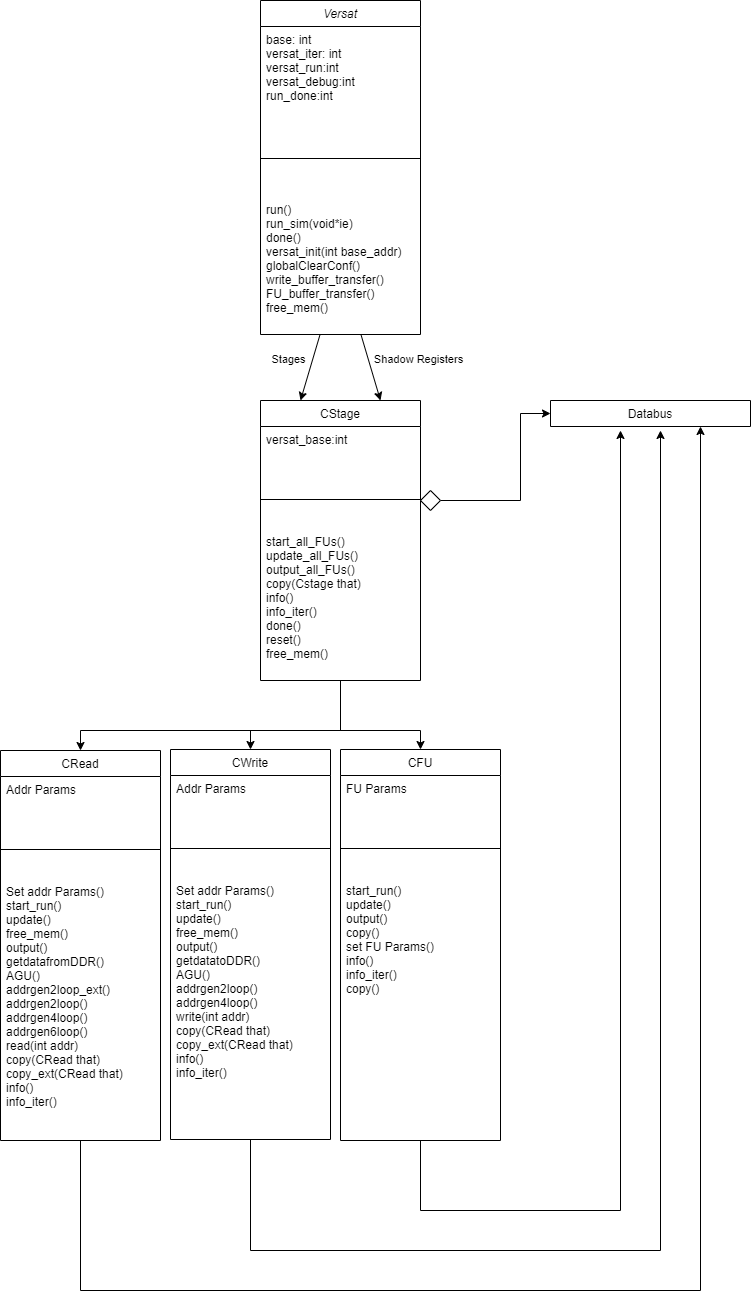
\includegraphics[width=0.8\textwidth]{Figures/VersatSimulatorDraw.drawio.png}
    \caption{Class Structure for the Versat Simulator}
    \label{figure:VersatSimulatorClass}
\end{figure} 


\subsection{Functional Units}

The following Table contains the functional units present in the simulator 
and is represented by 
"CFU" inFigure~\ref{figure:VersatSimulatorClass}. 
VI and VO represent CRead and CWrite 
classes respectively.



\begin{table}[!htbp]
    \centering
    \begin{tabular}{|ll|}
        \hline
        \textbf{Functional Unit}     & \textbf{Porpuse}  \\  \hline
        Read (VI) Mem Unit             & Reads from DDR and sends Data to databus            \\ \hline
        Write (VO) Mem Unit & Reads from databus and sends Data to DDR             \\ \hline
        MulAdd (MAC)    & Multiplication and Accumulate          \\ \hline
		Mul    & Multiplication     \\ \hline
		Alu    & Standard algorithmic and logic unit     \\ \hline
		AluLite    & Stripped down  algorithmic and logic unit     \\ \hline
		Barrel Shifter (BS) & Shifts to the right (division by 2) or to the left (multiplication by 2) \\ \hline
		Memory (Mem) & Sends/Receives data to/from the pipeline. \\ & Data is inserted through CPU communication   \\ \hline
        \end{tabular}
    \caption{Versat Simulator Functional Units}
    \label{table:versatsimfu}
    \end{table}

To add a new FU, it's as easy as creating a new class that CStage will use with
a run(), update(), output(), and copy() method. Of course, if it has variables needed to be defined
by the program, set param functions are also required. Using the simulator, hardware development
and program development can be parallelized to output a new program 
with more optimized performance.

In the next section, these methods will be explained in detail and 
their importance to the simulator.

\section{Simulation}

After the program that is running on the CPU finishes writing the configurations, it will call the run method of Versat.
InFigure\ref{figure:VersatSimulatorSequenceDiagram}, a sequence diagram is presented with the rundown
of a typical program that uses Versat Simulator.

\newpage
%Previously, a software API was made in a previous thesis~\cite{valter:deepversat}
%for Versat. To build on top of this several, software functions were added to make writing configurations to Versat
%easier.
\begin{figure}[!htbp]
    \centering
    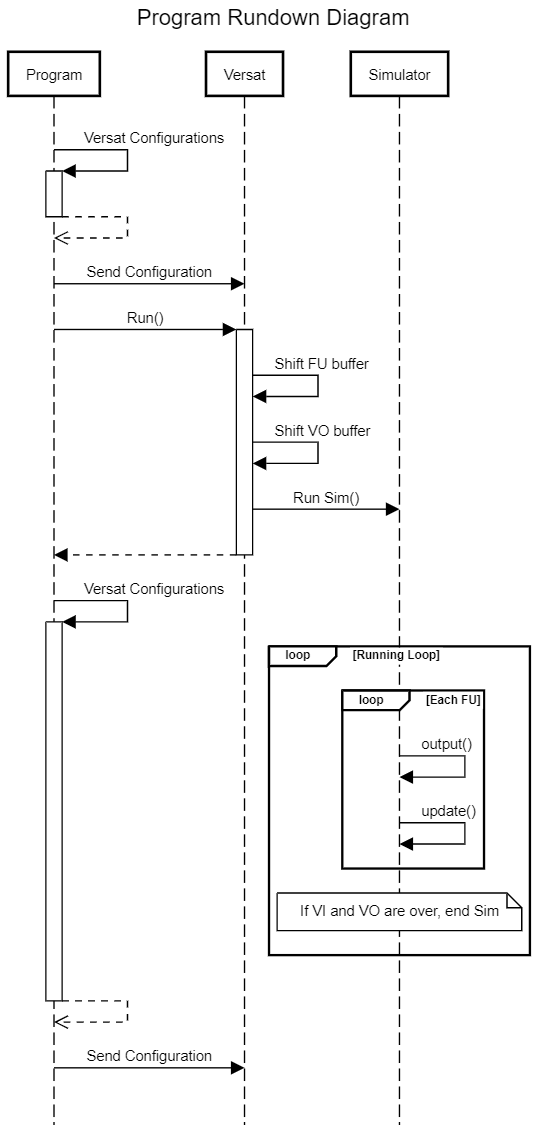
\includegraphics[width=0.7\textwidth]{Figures/versatsim.png}
    \caption{Sequence Diagram of a Program using Versat Simulator}
    \label{figure:VersatSimulatorSequenceDiagram}
\end{figure} 



\subsection{Run() Function}

In the software API for Embedded Versat, the run function would write to a shadow register,
which we can call "start", changing the value from zero to 1. 
Similarly, another register would
change the value to 0, which we can call "done". While this last register isn't turned to 1, 
Versat hasn't finished running with the 
previous configurations, so all that can be done is to write
configurations for future runs.

In the simulator, it works in a similar way to preserve compatibility 
as the goal is to have the same
programs run on software simulators and the FPGA.

\lstinputlisting[label=runfunctioncode,language=C++,frame=single,breaklines=true,firstline=222,lastline=245,caption= The Run function code]{./Code/Versat.cpp}

As we can see in the previous Listing, we reset the state variables of the simulator, then shift the VO and FU shadow registers.
This is done to simulate the pipeline delay in the FPGA. 
Because the data needs to come and go to the main memory (DDR),
One run cycle is used just for fetching data and writing data. 
Using a small example:
If a developer writes a configuration to do a 5x5 matrix multiplication, 
Versat will have to run three times.
Once to fetch data from memory, the second for the actual use of Versat 
and the final one is to get data onto memory.

In the simulator, this is done using the same class instances and 
copying the configuration values. On the hardware, it's several flip-flop registers in a row.
However, all these three stages can happen at once if you run multiple configurations in one program, e.g., running a CNN
through Versat will have at least one run per layer. 
So, if it has five layers, Versat will have to run 5+2 times. The last two times are done to
flush the Versat of any data.

After the shift, a new thread is created to run the simulator in parallel 
with the configurations,
having the same behavior as the hardware.

\subsection{Start() Method}

At the beginning of the configuration run, the method "start run" of 
all FUs and memories are started.
In this function, several functional units will have their state variables reset, such as VI, VO, and MAC FU.

\subsection{Databus}

The databus on Versat is a simple array that holds all the outputs of the functional units.
The array's data type (versat\_t) depends on the width of Versat, which is part of the configuration file.
Using higher width, e.g., 64 bits, is useful for the single instruction, multiple data (SIMD) 
applications but requires the functional units to be adapted.
For the purpose of this thesis, 16 bits and 32 bits are used depending 
on the neural network and how it is optimized.

When the Versat is instanced in the program, the functional units constructor will point
to the correct position of the databus as referenced in the following figure.

As mentioned inFigure\ref{figure:deepversatarch} from chapter \ref{chapter:Background}, section \ref{sector:DeepVersat}, 
each functional unit will be able to access the output from the functional units of the
current stage and previous. Software-wise, each stage will be pointing to a part of the databus.  

% INSERT FIGURE HERE


\subsection{Update() and Output() Method}


The update method's goal is to update the functional unit's value on the databus. 
Each functional unit has a pipeline delay to output or has a run delay configured, 
like the memories or MAC.

Meanwhile, the output method's goal is to, based on the inputs from the databus, calculate the result from
 the functional unit.

 For computing functional units such as the MAC or the ALU, this means reading from the databus for operands A and B
 and performing the selected operation. For the read memory (VI), it will output an address on the mem
 and performs a read operation. For the write memory, it will output an address and performs a write operation.

 In the Listing\ref{listing:fu}, the code of the Mul functional unit is used as an example.

 \newpage
 \lstinputlisting[label=listing:fu,language=C++,frame=single,breaklines=true,firstline=21,lastline=65,caption=Update and Output method of Mul]{./Code/mul.cpp}


\subsection{Copy() and Info() Method}

Finally, the last two functions of the simulator are copy() and info(). The former primary purpose is to copy the configuration parameters from one instance to another,
used mainly at the beginning of the run to simulate the shadow registers.
Meanwhile, the info method is a state printing function that outputs a string with the complete data of the current iteration,
this way, there will be an output file iteration by iteration to check the progress of the simulation, just like in a hardware simulator.

\lstinputlisting[label=listing:fu,language=C++,frame=single,breaklines=true,firstline=572,lastline=584,caption=Info output for the MAC functional unit]{./Code/versat_iter22.txt}
